\documentclass[crop,tikz]{standalone}
\usetikzlibrary{%
    arrows,
    arrows.meta,
    backgrounds,
    calc,
    decorations.pathreplacing,
    fit,
    matrix,
    positioning,
    scopes,
    shadows
}
\usepackage[linguistics]{forest}
\usepackage[charter]{mathdesign}
\tikzset{headarrow/.style = {-{Latex[length=.5em]}}}
\tikzset{move/.style = {dashed,blue,headarrow}}

\newcommand{\mlex}[2]{\ensuremath{\textrm{#1} ::\thinspace \mathrm{#2}}}
\newcommand{\fsel}[1]{\ensuremath{\mathrm{#1^+}}}
\newcommand{\fcat}[1]{\ensuremath{\mathrm{#1^-}}}
\newcommand{\flcr}[1]{\ensuremath{\mathrm{#1^+}}}
\newcommand{\flce}[1]{\ensuremath{\mathrm{#1^-}}}
\newcommand{\fadj}[1]{\ensuremath{\mathrm{#1^\sim}}}
\newcommand{\Merge}{Merge}
\newcommand{\Move}{Move}
\newcommand{\Adjoin}{Adjoin}

\begin{document}
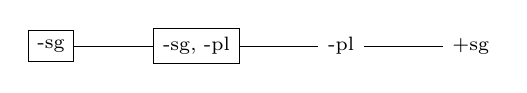
\begin{tikzpicture}
    \node[draw] (1) at (0,0) {$\text{-sg}$};
    \node[draw] (2) [right=of 1] {$\text{-sg, -pl}$};
    \node       (3) [right=of 2] {$\text{-pl}$};
    \node       (4) [right=of 3] {$\text{+sg}$};

    \foreach \Source/\Target in {1/2, 2/3, 3/4}
        \draw (\Source) to (\Target);
\end{tikzpicture}
\end{document}
